\documentclass{IEEEtran}
\usepackage{graphicx}
\usepackage{multirow}

\renewcommand\IEEEkeywordsname{Keywords}

\title{Survey Paper}
\author{
  Arvind Sudarshan,
  \and
  Chatane Shree,
  \and
  Eksambekar Yash,
  \and
  Gadkari Gaurav
}

\begin{document}

  \maketitle

  \begin{abstract}
  \end{abstract}
  \begin{IEEEkeywords}
  \end{IEEEkeywords}

  \section{Introduction}

  \section{Literature Survey}

    \subsection{Decentralised E-voting system based on Smart Contract by using Blockchain Technology \cite{9299581}}
      This Paper Explains the Difference between Ballot paper voting and Blockchain based decentralised casting For better integrity of the voting system.\\
      Here in Decentralised Blockchain System data like the name of voter or votes is saved on a decentralised ledger. This data neither be accessed nor be changed by any third party authority. Currency ballot paper is a widely used voting system worldwide. But this doesn't guarantee the correctness of the result Due to availability of data at a single resource. This problem is faced by a centralised voting system and is solved by Blockchain based voting systems. Here in Blockchain Technology the data is not stored on a central location but is allotted in different locations on different servers. The data which is distributed across each device connected to the blockchain using a peer-to-peer system.\\
      In the Decentralised E-voting system candidate registration is done before the voting process starts and then voters identity is verified before the creating account.In this system. The authorised person authenticates the voter and then blockchain ensures the double voting is not allowed.

    \subsection{Consensus algorithms used in Blockchain Technology \cite{8400278}}
      The Oxford Dictionary meaning of word consensus is: an opinion that all members of a group agree with. In Blockchain Technology every transaction must be verified and agreed upon by validators in the network before being inserted. To do so, various consensus algorithms have been defined for use. Some of the most commonly used consensus algorithms are Proof of Work (PoW) algorithm and Proof of Stake (PoS) algorithm.\\
      In this paper referenced, the authors have mentioned a few of the consensus algorithms used and their comparative analysis. Some High-profile consensus algorithms mentioned in the paper are Proof of Work (PoW), Ripple Protocol Consensus Algorithm (RPCA), Proof of Stake (PoS), Stellar Consensus Protocol (SCP), Delegated Proof of Stake (dPOS) and Proof of Importance (PoI). The authors have compared these algorithms on the basis of Security, Scalability and Power Consumption. A consensus algorithm characteristic comparison is provided in Table \ref{tab:tab1}.
      \begin{table*}
        \caption{Consensus Algorithm Comparision}
        \label{tab:tab1}
        \center
        \begin{tabular}{|l|llllll|}
          \hline
          \multicolumn{1}{|c|}{\multirow{2}{*}{Property}} & \multicolumn{6}{c|}{Algorithm Name}                                                                                                                                                                                                                                  \\ \cline{2-7} 
          \multicolumn{1}{|c|}{}                          & \multicolumn{1}{l|}{PoW}                             & \multicolumn{1}{l|}{RPCA}                         & \multicolumn{1}{l|}{PoS}                   & \multicolumn{1}{l|}{SCP}      & \multicolumn{1}{l|}{dPOS}                       & PoI                        \\ \hline
          Energy Saving                                   & \multicolumn{1}{l|}{No}                              & \multicolumn{1}{l|}{Yes}                          & \multicolumn{1}{l|}{Partial}               & \multicolumn{1}{l|}{Yes}      & \multicolumn{1}{l|}{Partial}                    & Yes                        \\ \hline
          Tolerated power of adversary                    & \multicolumn{1}{l|}{\textless{}25\% computing power} & \multicolumn{1}{l|}{\textless{}20\% faulty nodes} & \multicolumn{1}{l|}{\textless{}51\% stake} & \multicolumn{1}{l|}{Variable} & \multicolumn{1}{l|}{\textless{}51\% validators} & \textless{}50\% importance \\ \hline
          Example                                         & \multicolumn{1}{l|}{Bitcoin}                         & \multicolumn{1}{l|}{Ripple}                       & \multicolumn{1}{l|}{Cardano}               & \multicolumn{1}{l|}{Stellar}  & \multicolumn{1}{l|}{EOS}                        & NEM                        \\ \hline
        \end{tabular}
      \end{table*}

    \subsection{A Survey on Blockchain Technology: Evolution, Architecture and Security \cite{9402747}}
      This paper explains the Blockchain evolution, Architecture and security of blockchain.\\
      Blockchain 1.0 is associated with bitcoin technology founded by anonymous person Satoshi Nakamoto. Cryptocurrencies are considered the first application of Blockchain and have already been functional as a digital payment system on the Internet.\\
      Blockchain 2.0 is based on Smart Contracts. It is used for transferring assets like bonds, stocks, loans, Properties etc. Afterwards it is realised that that Blockchain can revolutionise for all the industries.\\
      Blockchain 3.0 provides a platform for development of secure applications for all the industries rather than only money exchange.It supports large scale interconnection using web technology.

    \subsection{Emergence of Blockchain \cite{zheng2018blockchain}}
      Blockchain gained most of its fame from bitcoin, a cryptocurrency.\\
      It is the backbone of bitcoin.The concept of blockchain was first proposed in 2008 and implemented a year later. Satoshi Nakamoto is dubbed as the creator of blockchain.Blockchain has several different characteristics like decentralisation, persistence, anonymity and auditability. Blockchain has various diverse applications other than bitcoin.Its ability to conduct transactions without banks make it a strong contender for online payments.

    \subsection{Blockchain types and their comparision \cite{8029379}}
      In Blockchain Technology, there exists three major types: Public blockchain, Consortium blockchain and Private blockchain. Since a network will have to be created, a comparison must be made on what kind of network must be used for the same. The types are compared on the basis of Consensus determination, Read permission, Immutability, Efficiency, whether it is centralised or not and the Consensus process. Depending upon the application, a developer must decide what kind of blockchain should be used. Table \ref{tab:tab2} shows a comparision between the types of blockchains.
      \begin{table*}
        \caption{Types of Blockchains}
        \label{tab:tab2}
        \center
        \begin{tabular}{|l|lll|}
          \hline
          \multicolumn{1}{|c|}{\multirow{2}{*}{Property}} & \multicolumn{3}{c|}{Types of Blockchain}                                                                                              \\ \cline{2-4} 
          \multicolumn{1}{|c|}{}                          & \multicolumn{1}{l|}{Public Blockchain}           & \multicolumn{1}{l|}{Consortium Blockchain}         & Private Blockchain            \\ \hline
          Consensus determination                         & \multicolumn{1}{l|}{All miners}                  & \multicolumn{1}{l|}{Selected set of nodes}         & One Organisation              \\ \hline
          Read permission                                 & \multicolumn{1}{l|}{Public}                      & \multicolumn{1}{l|}{Could be public or restricted} & Could be public or restricted \\ \hline
          Immutability                                    & \multicolumn{1}{l|}{Nearly impossible to tamper} & \multicolumn{1}{l|}{Could be tampered}             & Could be tampered             \\ \hline
          Efficiency                                      & \multicolumn{1}{l|}{Low}                         & \multicolumn{1}{l|}{High}                          & High                          \\ \hline
          Centralised                                     & \multicolumn{1}{l|}{No}                          & \multicolumn{1}{l|}{Partial}                       & Yes                           \\ \hline
          Consensus process                               & \multicolumn{1}{l|}{Permissionless}              & \multicolumn{1}{l|}{Permissioned}                  & Permissioned                  \\ \hline
        \end{tabular}
      \end{table*}

    \subsection{Characteristics of Blockchain \cite{viriyasitavat2019blockchain}}
      \begin{itemize}
        \item \textbf{Cost effective:} In traditional systems there is a need for a central agency to validate transactions. Blockchain is a peer to peer network(P2P). The absence of a central agency reduces the cost per transaction.
        \item \textbf{Persistence:} Blockchain has one important property of persistence, Each block has the ability to maintain its records. This helps in keeping the data tamper proof.
        \item \textbf{Validity:} The execution is not carried out every time. This system has three roles, proposer, acceptor, learner.
        \item \textbf{Anonymity \& Identity:} The centralised systems require to know you as a person. You need to register your identity proof with those authorities. Whereas with blockchain, the user data remains fairly anonymous.
        \item \textbf{Auditability:} The block added to the blockchain remains there forever. This helps in checking transaction history. In private blockchain the auditability is least and depends on the central entity. In permissioned blockchain there is a little bit of auditability. In public blockchain have the most auditability.
      \end{itemize}

    \subsection{A Framework to Make Voting System Transparent Using Blockchain Technology \cite{9787540}}
      This paper explains about the transparent voting system using blockchain technology. It reduces a lot of resources and efforts in the polling system. Unlike the traditional voting system which stores votes on a centralised system, blockchain based voting systems are not easily tampered. Blockchain provides a high level of security that can be trusted more than the previously used technologies.\\
      Here voters need to complete verification into the voting management system. The nation's database is integrated with the system's database to keep voters’ integrity. For every vote, a transaction is generated against the voter’s National ID then the transaction is saved in blockchain. After casting a vote his/her vote coin is used. After casting vote blockchain verifies his voting system by comparing with the national voting ids. Then miners analyse them to remove malicious votes before adding them to the chain.

    \subsection{An Architecture of Blockchain based Voting System \cite{angsuchotmetee2019blockvote}}
      The paper proposes a Blockchain-based voting system called BlockVOTE. It focuses on keeping the voting system secure and trustable using consensus handling mechanisms. The paper covers Traditional Ballot based Voting systems and Electronic based Voting Systems with both their issues. In the proposed architecture, the paper defines upon processes Poll Creation, Voting and Result Tallying. Authors of the paper implemented the system using Ethereum and HyperLedger and compared the results. The system will have the following actors: Poll Creator, Contract Handler and Voter performing tasks of Poll Creation, Contract creation and deployment and Voting.

    \subsection{Scalability of Blockchain \cite{8962150}}
      \begin{itemize}
        \item \textbf{Bitcoin-Cash:} It is another form of cryptocurrency. It is the hard fork from bitcoin’s codebase. The main idea is to solve the scalability issue of the blockchain. The solution here is to increase the block size while keeping the block interval the same. The block size of bitcoin was 1 MB, but now bitcoin and bitcoin cash has increased its blocksize to 8 MB. After that there was further increase in the block size of bitcoin cash to 32 MB.However we cannot increase the blocksize infinitely as there is a limitation to the intra-blockchain bandwidth. The larger block sizes may also lead to the problems of centralization.
        \item \textbf{Block compression:} In compact block relay technique the data structure is little altered. The block contains the headers and some short transaction IDs,  used to match transactions already available to the receivers. The compact block messages are sent and receivers process these messages. The node A sends the compact block to the node B. When node B receives the compact block it calculates the transaction IDs in the memory pool and matches it with the transactions IDs in the compact block. If all transactions are available the block is reconstructed if not node B sends the getblocktxn message to node A to receive all transaction data. After that the block is constructed.In low bandwidth relaying the compact blocks are sent only if the request is made.
        \item \textbf{Storage scheme Optimization:} This scheme has a consensus unit. It has a number of nodes in it. The blocks of the whole chain are assigned to a single unit. This reduces the total query cost.\\Jidar is another approach. The main idea is to store only relevant data they are interested in. Small part of the data is stored including the relevant transactions and the merkel branch. If at all we need all the block data, the nodes ask the other nodes and the complete blocks are constructed out of it. There needs to be some incentives for other blocks to help the block asking for the complete data.
      \end{itemize}

    \subsection{An Empirical Analysis Of Using Blockchain Technology In E-Voting Systems \cite{9681365}}
      This paper discusses the difference between a centralised e-voting system and a blockchain based e-voting system in terms of performance and security. Both systems were designed to have similar interfaces. The only difference between them was the systems used to design the backend. With blockchain based systems, the users needed to use their digital wallet's private key as their credentials to connect to the network. If all the conditions of the contact are satisfied, a new block is created, processed and then added to the blockchain, which serves as the database for this system. The centralised system required users to log in with their voter ID. The votes are processed by the server and stored in a database, which automatically counts the number of votes for each candidate.  Results showed that BEVS is slightly slower than CEVS. This is due to the additional processes of block validation and creation while using a local private blockchain, it processes requests faster than a public blockchain network.  However, the BEVS is more reliable when it comes to efficiency as it has a zero error rate compared to the CEVS with its errors. through the internal server. However, the rate at which the BEVS works can be affected even by heavy loads. The BEVS is also proving to be a more secure electronic voting system with fewer identified vulnerabilities.
      
    \subsection{Blockchain Based E-Voting System: Open Issues and Challenges \cite{9670245}}
      This paper analyses current research on blockchain electronic voting systems and identifies issues in it. E-Voting defines the process that uses electronic tools in the process of elections for voting and counting purposes. The procedure for electronic voting varies from country to country. which may include voting machines on polling stations, centralised accounting of paper bills and voting on the Internet. In many countries, centralised calculations are used. Sometimes, however, they also use electronic voting machines in places of voting. However, the use of the internet is minimal. In particular, electronic approaches have been tested in several places and problems with security and reliability were noted. This paper also talks about several factors that makes an e-voting system secure like,
      \begin{enumerate}
        \item \textbf{Anonymity:} Any correlation between registered voters and voter identities shall be anonymous.
        \item \textbf{Auditability and Accuracy:} The results should be accurate and should precisely correspond to the voter sentiment.
        \item \textbf{Democracy/Singularity:} Every eligible person should be able to vote. There shall be no duplication of votes.
        \item \textbf{Vote Privacy:} No one should be able to associate a particular vote to an individual.
        \item \textbf{Robustness and Integrity:} It ensures that registered voters will abstain without problems or encourage others to cast their legitimate votes for themselves.
        \item \textbf{Transparency and Fairness:} It means that no one outside the people involved with the counting process can find out about the results before they are announced.
        \item \textbf{Availability and Mobility:} The systems should always be available during the electoral process.
        \item \textbf{Verifiable Participation/Authenticity:} The authorities should be able to check if someone abstained from voting.
        \item \textbf{Recoverability and Identification:} It should be able to track and restore data in order to avoid attacks or data losses.
      \end{enumerate}
      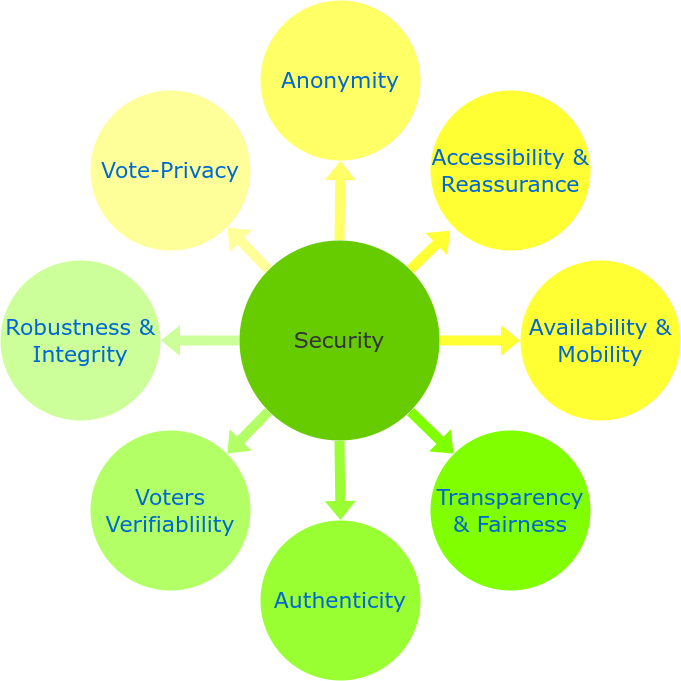
\includegraphics[width=\linewidth]{Resources/SecurityFlower.png}
      A blockchain includes the following components:
      \begin{enumerate}
        \item \textbf{Node:} User or computer within the blockchain network.
        \item \textbf{Transaction:} The most fundamental part of a blockchain system.
        \item \textbf{Block:} A data structure used for storing the transactions.
        \item \textbf{Chain:} A sequence of blocks in a specific order.
        \item \textbf{Miners:} Specific nodes which perform the block verification process.
        \item \textbf{Consensus:} A set of rules and arrangements to carry out blockchain operations.
      \end{enumerate}
      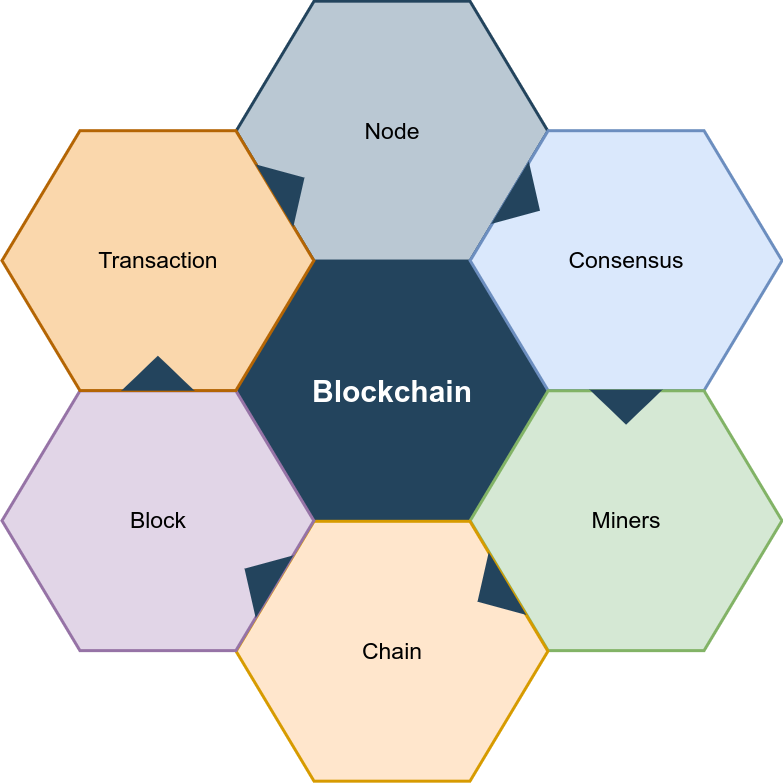
\includegraphics[width=\linewidth]{Resources/BlockchainCycle.png}
      Issues:
      \begin{enumerate}
        \item Scalability and Processing Overheads: For a small number of users, blockchain works well. However, when the network is used for large-scale elections, the number of users increases, which leads to an increase in the cost and time to complete the transaction.
        \item User Identity: The blockchain uses pseudonyms as the username. This strategy does not provide complete confidentiality and secrecy. Since transactions are publicly available, the identity of the user can be discovered by examining and analysing them.
        \item Transactional Privacy: In blockchain technology, it is difficult to ensure the anonymity of transactions and confidentiality. However, an electoral system requires transaction secrecy and anonymity due to the presence of transactions.
        \item Energy Efficiency:  Blockchain includes energy-intensive processes such as protocols, consensus, peer-to-peer communication, and asymmetric encryption. Appropriate energy efficient consensus methods are required for blockchain-based e voting.
        \item Acceptableness Although blockchain is accurate and secure, people's confidence and trust are critical components of effective electronic voting on the blockchain. The complexity of the blockchain can make it difficult for people to accept blockchain-based e-voting and could pose a major obstacle to the ultimate adoption of blockchain-based e-voting as mainstream.
        \item Political Leaders’ Resistance Central governments such as electoral bodies and government bodies will be diverted from blockchain-based e voting. As a result, political leaders who profit from the existing electoral process are likely to oppose the technology because blockchain will increase social resistance through decentralised autonomous organisations.
      \end{enumerate}
    
    \subsection{Analysis of Blockchain Solutions for E-Voting: A Systematic Literature Review \cite{9812616}}
      This paper reviews the latest innovations in the  blockchain based e-voting system to understand their particulars and compares them with each other as well as the traditional voting process. Various blockchain based e-voting applications here are being compared based on many parameters like  implementations used, algorithms used, voter identification methods, vote encryption methods, how they fare against attacks and their security properties. After comparing these based on the said factors, limitations and constraints of these systems. Even though the blockchain based systems for voting may be in their initial phases, they offer an interesting solution to the problems of traditional voting.

  \section{Outcome of Literature Survey}

  \section{Conclusion}

  \bibliographystyle{ieeetr}
  \bibliography{References}

\end{document}